In this chapter, we presented numerical simulations conducted in order to characterize and compare the performance of the time-frequency interpolation method of \citet{Thiergart2013} to our proposed parametric interpolation method.
Following the simulation framework laid out in \chapref{chap:06_Simulation_Framework}, we simulated simple incident sound fields consisting of a two-microphone array and a single point-source, varying source distance and azimuth, as well as microphone spacing and listener position.
We first explored basic properties of the time-frequency method by computing the effective frequency responses induced by translation via the method across source azimuths.
Then, we conducted a more comprehensive analysis of the methods by computing, for a wide range of conditions, the metrics enumerated in \secref{sec:06_Simulation_Framework:Metrics} for sound level, spectral coloration, source localization, and diffuseness.
The analyses presented in this chapter yielded the following findings:
\begin{itemize}
\item the time-frequency method yields virtually exact sound levels for all conditions, and is particularly superior to the proposed method for interior sources;
\item the time-frequency method yields significantly larger spectral errors than the proposed method for microphone spacings larger than approximately $0.5$~m;
%\item that these larger errors will be perceptible as increased coloration is reinforced by established psychoacoustic results;
%\item while the precise origin of this coloration remains unclear, it may well be related to the presence of wider (but shallower) notches in the frequency responses induced by the time-frequency method compared to those induced by the proposed method;
\item the time-frequency method yields significantly smaller localization errors than the proposed method for interior sources with microphone spacings larger than approximately $1$~m; and
\item the time-frequency method does not sufficiently reproduce the diffuseness of a sound field, whereas the proposed method yields virtually exact diffuseness for almost all conditions.
\end{itemize}

%\subsection{Practical implications}
Taken together, the findings presented in this chapter suggest that the time-frequency method and the proposed method may each be more suitable in different practical domains.
For the present discussion, we define the following practically-relevant ``axes'':
\begin{enumerate}
\item the \textit{sparsity} of the microphone array, i.e., the size of the desired navigable region relative to the number of available microphones (e.g., $\sim\Delta/2$);
\item the \textit{intimacy} of the sound sources, i.e., the proximity of the sources to the navigable region (e.g., $\sim1/\gamma$); and
\item the \textit{complexity} of the sound field, i.e., the total number of sources and/or the reverberance of the recording environment.
\end{enumerate}
%These axes are illustrated in \figref{fig:09_Thiergart_Comparison:Practical_Axes}.
While the first two of these axes can be easily related to microphone spacing and normalized source distance, respectively, the third axis has not been directly explored here.
However, based on the construction of the time-frequency method, we speculate that this method may have difficulties accommodating multiple sources since, at each time-frequency bin, only a single point-source is created (see \secref{sec:03_Navigation_Techniques:Thiergart_Method}).
Consequently, the capability of this method to accurately reproduce multiple sources warrants further study.

%\begin{figure}[tb]
%	\includegraphics[width=\textwidth]{extras/figures/Practical_Axes_Diagram.pdf}
%	\caption{Illustration of the three practically-relevant axes defined in the text:
%	the sparsity of the microphone array,
%	the intimacy of the sound sources,
%	and the complexity of the sound field.
%	Empty circles indicate microphones,
%	filled circles indicate sources,
%	the filled rectangle indicates a scattering body,
%	and the hatched line indicates a reflective surface.}
%	\label{fig:09_Thiergart_Comparison:Practical_Axes}
%\end{figure}

Nevertheless, below, we identify several general principles with which to choose between the two methods in various applications spanning these axes:
\begin{enumerate}
% sparsity axis
\item[1a.] With a sparse microphone array (e.g., when covering a large room with only a few microphones), the time-frequency method will generally yield superior localization accuracy, whereas the proposed method will incur less spectral coloration.
\item[1b.] With a dense microphone array, the methods perform comparably to each other (i.e., neither method is particularly superior) in terms of localization accuracy and spectral coloration.
% intimacy axis
\item[2a.] When recording primarily intimate sources (e.g., an immersive recording of a small group of musicians), the time-frequency method will yield superior localization accuracy and will likely better convey source distance information (due to its accurate reproduction of sound level), whereas the proposed method will again incur less spectral coloration.
\item[2b.] When recording primarily distant sources (e.g., when covering the audience section only of a concert hall), the proposed method will yield smaller spectral and localization errors.
% complexity axis
\item[3a.] For an acoustically complex sound field (e.g., in a room with highly reflective surfaces and/or many scattering bodies), the proposed method is likely more suitable as it more accurately reproduces diffuseness and, potentially, the time-frequency method will fail to adequately reproduce many sources.
\item[3b.] For an acoustically simple sound field (e.g., an outdoor recording of a park with sparsely distributed sources), the time-frequency method will likely yield superior localization accuracy, and its deficiency in diffuseness will be less problematic.
\end{enumerate}

% Parameters:
% sparsity of microphone array: size of desired navigable region / number of microphones
% intimacy of sound field: presence of important sources with \gamma < 1
% sound field complexity: number of sources * reverberance of environment

% order of microphones
% movement of sources
% most important attributes: sound quality vs. spatial accuracy

While these principles specify the superior method for any given practical domain, another way of summarizing the results presented in this chapter is to determine the domains, in terms of these practical axes, over which each method yields \textit{accurate and superior} performance.
As we did not explore the complexity axis explicitly, here we omit that axis and focus only on the sparsity of the microphone array and the intimacy of the sources.
Additionally, since the level and diffuseness results are relatively straightforward (see \figreftwo{fig:09_Thiergart_Comparison:Level_Errors}{fig:09_Thiergart_Comparison:Diffuseness_Errors}, respectively), we omit those metrics as well.

Using the errors plotted in \figreftwo{fig:09_Thiergart_Comparison:Spectral_Errors}{fig:09_Thiergart_Comparison:Localization_Errors}, we first identify, for each method, regions of low coloration ($\rho_\eta < 3$~dB) and regions of accurate localization ($e_\nu < 10^\circ$).
We then determine the regions in which each method performs a) more accurately than that error limit and b) more accurately than, or at least comparably to, the other method.
These regions are sketched in \figref{fig:09_Thiergart_Comparison:Region_Plots}.

\begin{figure*}[t]
	\centering
	\begin{subfigure}[b]{0.49\textwidth}
		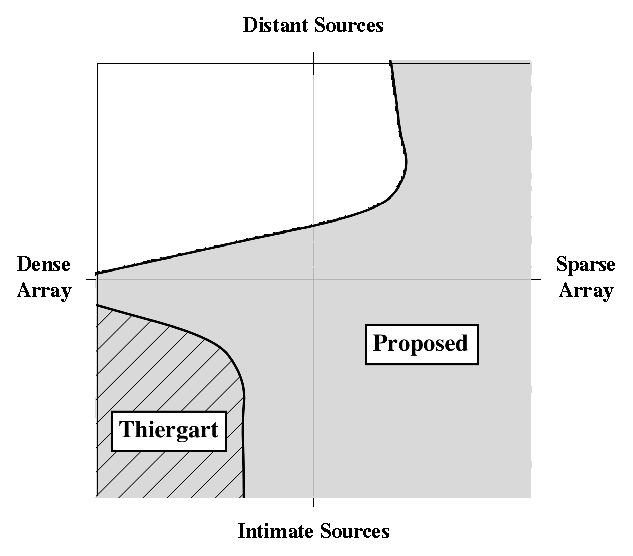
\includegraphics[width=\textwidth]{09_thiergart_comparison/figures/Coloration_Region_Plot}
		\caption{Coloration}
		\label{fig:09_Thiergart_Comparison:Region_Plots:Coloration}
	\end{subfigure}
	\hfill
	\begin{subfigure}[b]{0.49\textwidth}
		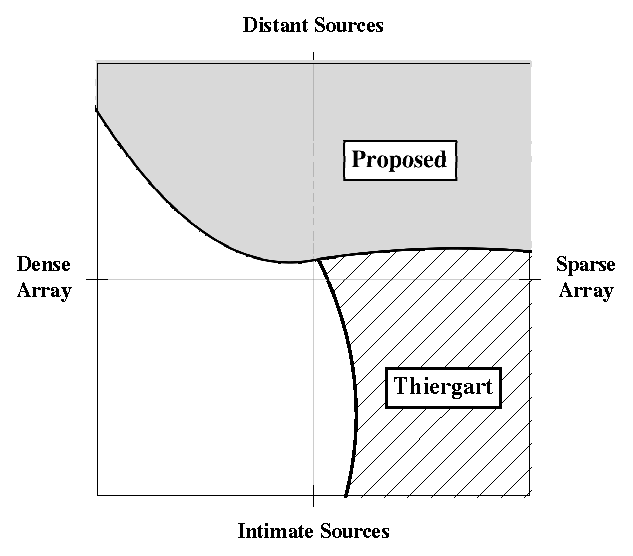
\includegraphics[width=\textwidth]{09_thiergart_comparison/figures/Localization_Region_Plot}
		\caption{Localization}
		\label{fig:09_Thiergart_Comparison:Region_Plots:Localization}
	\end{subfigure}
	
	\caption[Region plots of practical applicability of each interpolation method.]{
	Region plots illustrating accurate and superior methods in terms of spectral coloration (left panel) and localization accuracy (right) across practical applications with varying microphone array sparsity (horizontal axis) and sound source intimacy (vertical).
	The gray filled regions correspond to the proposed method and
	the hatched regions correspond to the time-frequency method of \citet{Thiergart2013}.
	Regions that are both filled and hatched indicate that the methods perform comparably;
	empty regions indicate that neither method satisfies the specified error limit.}
	\label{fig:09_Thiergart_Comparison:Region_Plots}
\end{figure*}

From these plots, we see that, in applications with distant sources and with a sparse microphone array, the proposed method yields accurate and superior performance in both coloration and localization.
Furthermore, for most applications with a sparse microphone array or with intimate sources, the proposed method yields accurate and often superior spectral coloration performance, and for most applications with distant sources, the proposed method yields accurate and superior localization performance.
The time-frequency method, however, yields accurate spectral coloration performance only for applications with a dense microphone array and with intimate sources, and the method yields accurate and superior localization performance only for applications with a sparse microphone array and with intimate sources.
Consequently, in such applications (with both a sparse microphone array and with intimate sources), the time-frequency method yields improved localization but degraded coloration performance compared to the proposed method.

% a more general discussion of practical things
A practical advantage of the time-frequency method is that it only requires first-order ambisonics microphones (which tend to be significantly less expensive than higher-order ones and require fewer recording channels, preamplifiers, etc.).
However, as shown in \secref{sec:08_Proposed_Method:Order_Dependence}, the performance of the proposed method does not vary significantly with order, so similar performance to that shown in this chapter would be achieved even with only $L_\text{in} = 1$.
Also, as mentioned in \secref{sec:09_Thiergart_Comparison:Simulations}, the time-frequency method fails to triangulate sources with azimuths of $|\varphi_0| = 90^\circ$.
While, in practice, a source azimuth of exactly $\pm 90^\circ$ is virtually impossible (e.g., due to positioning errors, noise, etc.), this does suggest that the triangulation calculation (see \eqnref{eq:03_Navigation_Techniques:Source_Triangulation}) may be very sensitive to small changes in azimuth near these extremes.
This issue might be easily avoided, however, by using $P > 2$ microphones arranged in a triangular or rectangular configuration, for example.

While the evaluation presented in this chapter has been purely numerical, we hope that the practical recommendations enumerated above will facilitate real-world implementations of these navigational methods.
Ideally, the conclusions drawn from these analyses will be borne out by future experimental investigations.
To that end, in the following chapter, we present an experimental validation of our numerical simulation framework (from \chapref{chap:06_Simulation_Framework} but which has been use throughout \chaprefthru{chap:07_Characterization_Extrapolation}{chap:09_Thiergart_Comparison}), which will serve to ground the findings presented throughout this thesis in experimentally measured data.